\section{Las im�genes de piel y sus caracter�sticas}

\subsection{Procesamiento digital de im�genes}
\begin{frame}
	\frametitle{Procesamiento digital de im�genes}
	Este problema se enmarca en el procesamiento digital de im�genes. \pause
	Algunas dificultades: \pause
	\begin{itemize}
		\item Escala \pause
		\item Elementos que afectan la imagen \pause
		\item Espacio de color \pause
		\item Detecci�n de bordes \pause
		\item Detecci�n de c�rculos \pause
		\item Falsos positivos y falsos negativos \pause
		\item Detecci�n de la piel
	\end{itemize}
\end{frame}

\begin{frame}
	\frametitle{Escala}
	\begin{tabular}{cc}
		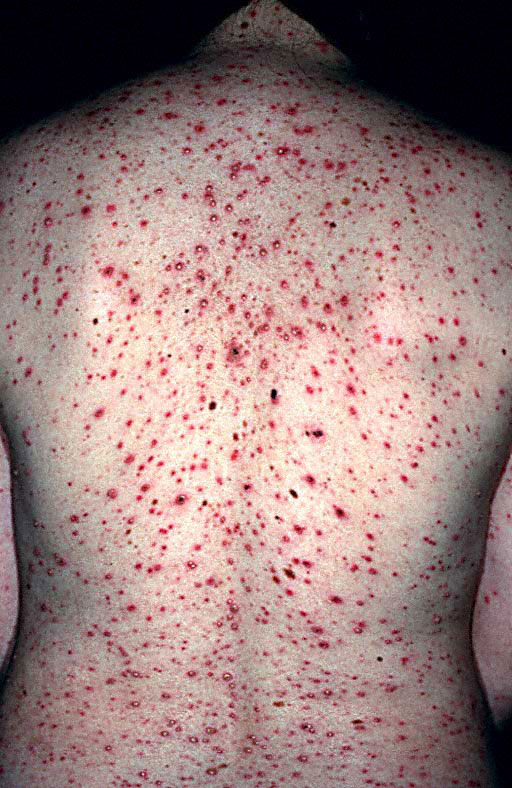
\includegraphics[width=1.7in]{../Imagenes/U.Iowa/Varicela/chicken_pox_picture_01.jpg} &
		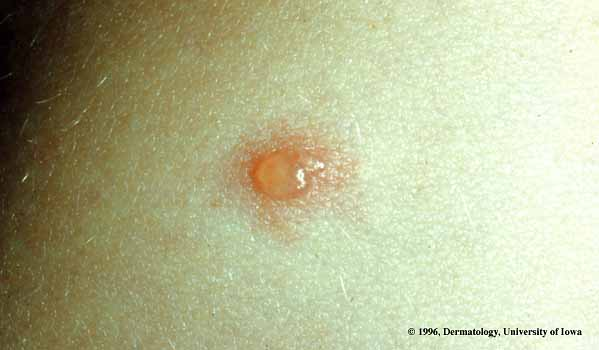
\includegraphics[width=1.7in]{../Imagenes/U.Iowa/Varicela/Varicel-02.jpg}
	\end{tabular}
\end{frame}

\begin{frame}
	\frametitle{Elementos que afectan la imagen}
	Problemas
	\begin{itemize}
		\item Ruido
		\item Imperfecciones de la piel
		\item Luces y sombras
		\item Elementos ajenos
	\end{itemize}
	T�cnicas
	\begin{itemize}
		\item Ecualizaci�n del histograma (Contrast-limited adaptive histogram equalization)
		\item Reducci�n del ruido o suavizaci�n utilizando un filtro gaussiano
	\end{itemize}
\end{frame}
